\documentclass[parskip=full]{scrartcl}
\usepackage[top=2.5cm, bottom=2.5cm, left=2.5cm, right=2.5cm]{geometry}
\usepackage[utf8]{inputenc}
\usepackage[T1]{fontenc}
\usepackage[german]{babel}
\usepackage{hyperref}
\usepackage[toc, nonumberlist]{glossaries}
\usepackage{graphicx}
\usepackage{enumitem}
\usepackage{float}
\usepackage{color}

\hypersetup{
  colorlinks=false,
  linktoc=all,
  hidelinks,
}

%!TEX root = Pflichtenheft.tex

\newglossaryentry{Dockerimage}
{
  name=Dockerimage,
  plural=Dockerimages,
  description={Ein Container mit Programmen, der unabhängig vom zugrunde liegenden Betriebssystem gleichbleibende Bedingungen herstellt}
}

\newglossaryentry{Fertigungssimulation}
{
  name=Fertigungssimulation,
  plural=Fertigungssimulationen,
  description={Darstellung der Industrieanlage und Simulieren des Verhaltens}
}


\newglossaryentry{GUI}
{
  name=GUI,
  plural=GUIs,
  description={Die grafische Benutzerumgebung des Programms, welche vom Bediener gesehen wird}
}

\newglossaryentry{Industrial Data Space}
{
  name=Industrial Data Space,
  plural=Industrial Data Spaces,
  description={Eine Infrastruktur zum Austausch von Daten in der Industrie}
}

\newglossaryentry{Jitter}
{
  name=Jitter,
  description={Simulation von variierenden Werten, um näher an echten Anlagen zu liegen}
}

\newglossaryentry{Makro}
{
  name=Makro,
  plural=Makros,
  description={Eine aufgezeichnete Folge von Einstellungen, die gesetzt werden. Wird benutzt, um einen komplexeren Ablauf in der Anlage zu simulieren}
}

\newglossaryentry{OPC UA}
{
  name=OPC UA,
  plural=OPC UA,
  description={Ein Protokoll zur Übertragung von Daten und Steuersignalen von Industrieanlagen}
}

\newglossaryentry{Produktionsanlage}
{
  name=Produktionsanlage,
  plural=Produktionsanlagen,
  description={Großmaschinen, wie sie in der Industrie eingesetzt werden. Hier symbolisiert durch Tanks mit Flüssigkeiten}
}

\newglossaryentry{Sensordatum}
{
  name=Sensordatum,
  plural=Sensordaten,
  description={Ausgabewert eines simulierten Sensors wie Temperatur oder Durchflussmenge}
}

\newglossaryentry{Systemadapter}
{
  name=Systemadapter,
  plural=Systemadapter,
  description={Konvertiert die Daten eines Gesamtsystems (hier Industrieanlage) in ein anderes Format}
}

\newglossaryentry{TCP/IP Verbindung}
{
  name=TCP/IP Verbindung,
  plural=TCP/IP Verbindungen,
  description={Ein Protokoll zum Datenaustausch über das Internet}
}

\newglossaryentry{Uberwachungskonsole}
{
  name=Überwachungskonsole,
  plural=Überwachungskonsolen,
  description={Anzeige der Sensorwerte der Fertigungssimulation}
}

\newglossaryentry{Wrapper}
{
  name=Wrapper,
  plural=Wrapper,
  description={Programm, das ein anderes Programm umgibt und auf Ereignisse im umgebenen Programm reagieren kann}
}
\makeglossaries

\title{OSIP - Pflichtenheft}
\subtitle{\gls{OPC UA} Simulator for Industrial Plants}
\author{
    M. Armbruster\\
    D. Kahles\\
    H. Lehmann\\
    M. Schwarzmann\\
    N. Wilhelm
}

\begin{document}
\maketitle

\vspace{20px}
\begin{center}
  
\includegraphics[scale=0.4]{../icon.png}
\end{center}
\pagebreak
\tableofcontents
\pagebreak

\section{Einleitung}
In der heutigen Zeit dringt die Vernetzung in immer neue Bereiche vor. So auch in die Industrie und ihre Fertigungsprozesse.
Dabei soll das Projekt \gls{Industrial Data Space} helfen, einen Datenraum zu erzeugen, der Datensicherheit, Datensouveränität und
Transparenz bietet. Auf diese Weise soll dazu beigetragen werden, die Industrie 4.0 voranzutreiben und somit durch Vernetzung von
Maschinen, Computern und Menschen die Leistungsfähigkeit der Industrie zu erhöhen und auf die Zukunft auszurichten.
Dabei macht es das auf \gls{TCP/IP} basierende Kommunikationsprotokoll \gls{OPC UA} möglich, dass Maschinen miteinander kommunizieren.

Die hier vorgestellte Simulation ermöglicht es, die Vorteile der Vernetzung von Maschinen mit \gls{OPC UA} interaktiv
zu demonstrieren, um Industriekunden von den neuen Möglichkeiten zu überzeugen. Die Hauptkomponenten sind eine \gls{Fertigungssimulation}
mit \glslink{OPC UA Server}{OPC UA Servern} und eine \gls{Uberwachungskonsole} mit \glspl{OPC UA Client}, die jeweils eine graphische
Benutzeroberfläche (\gls{GUI}) enthalten und auf getrennten Computern laufen können. Sie kommunizieren lediglich über \gls{OPC UA}.

\begin{figure}[H]
	\centering
	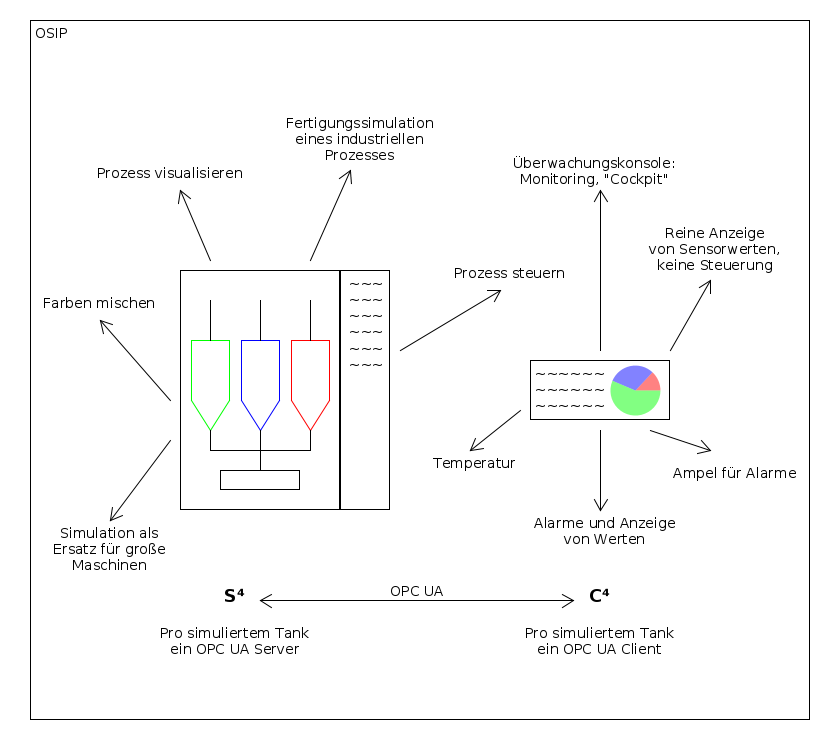
\includegraphics[scale=0.5]{../system-sketch.png}
	\caption{Systemskizze}
\end{figure}

Dieser Zusammenhang ist in der Systemskizze (siehe Abbildung 1) verdeutlicht. Links ist die \gls{Fertigungssimulation} bzw. ihre \gls{GUI} skizziert.
Dar\"uber wird die Simulation gesteuert. Darunter sind die vier verschiedenen \glspl{OPC UA Server} (S) angedeutet.
Rechts ist die \gls{Uberwachungskonsole} zu sehen. Unter ihr und zu ihr geh\"orend sind die vier \glspl{OPC UA Client} (C).
Der Doppelpfeil zwischen den \glslink{OPC UA Server}{OPC UA Servern} und \glspl{OPC UA Client} verdeutlicht, dass die Kommunikation
zwischen den beiden Programmen ausschließlich auf Ebene von \gls{OPC UA} abl\"auft.

In der GUI der \gls{Fertigungssimulation} wird eine \gls{Produktionsanlage} dargestellt.
Drei Tanks werden mit je einer farbigen Flüssigkeit gefüllt. Die Flüssigkeiten werden über Rohre in einen weiteren Tank geleitet,
in dem diese dann durch einen Motor gemischt werden. Daten und Werte der \gls{Produktionsanlage} werden ebenfalls angezeigt.
Dazu gibt es die Möglichkeit, die \glspl{Prozessvariable} der \gls{Produktionsanlage} zu konfigurieren. Dies geschieht beispielsweise dadurch, dass man
Zu- und Abflussmengen einstellt. Die visuelle Darstellung passt sich an die Konfiguration an.

Die \gls{Uberwachungskonsole} liest die Daten der \gls{Fertigungssimulation}, stellt sie optisch ansprechend dar und kann Alarme
anzeigen, die von \glspl{OPC UA Server} empfangen werden. Sie dient somit als reines Monitoring-Werkzeug
und hat keinen Einfluss auf die \gls{Fertigungssimulation}.

\pagebreak
\section{Zielbestimmung}
OSIP dient dem Ziel, die Funktion von \gls{OPC UA} zu demonstrieren, ohne eine konkrete \gls{Produktionsanlage}
benutzen zu müssen. Somit kann beim Kunden das Protokoll flexibler vorgestellt werden. Hierzu soll OSIP
sowohl eine \gls{Produktionsanlage} simulieren und deren Status graphisch darstellen, als auch auch eine \gls{Uberwachungskonsole}
bereitstellen, die mit Hilfe von \gls{OPC UA} die \glspl{Sensordatum} der \gls{Produktionsanlage} abfragt.\\

\subsection{Musskriterien}
\subsubsection{Allgemein}
\begin{itemize}
  \item Die simulierte \gls{Produktionsanlage} ist ein chemischer Produktionsprozess mit vier Tanks und Flüssigkeiten, die darin gemischt werden.
  \item Die Kommunikation zwischen \gls{Uberwachungskonsole} und \gls{Fertigungssimulation} findet ausschließlich \"uber
  \glspl{OPC UA Server} auf Seiten der \gls{Fertigungssimulation} und \glspl{OPC UA Client} auf Seiten der \gls{Uberwachungskonsole} statt.
  \item Die \gls{Fertigungssimulation} mit den \glslink{OPC UA Server}{OPC UA Servern} und die \gls{Uberwachungskonsole} mit den \glspl{OPC UA Client} ist auf dem selben oder auch auf getrennten Rechnern lauffähig.
\end{itemize}

\subsubsection{Fertigungssimulation}
\begin{itemize}
  \item Die \gls{Fertigungssimulation} enth\"alt eine schematische Darstellung der simulierten \gls{Produktionsanlage}.
  \item In der \gls{GUI} der \gls{Fertigungssimulation} kann der Benutzer die simulierte \gls{Produktionsanlage} steuern.
  \item Die \gls{Fertigungssimulation} aktualisiert die \glspl{Sensordatum} in den \glslink{OPC UA Server}{OPC UA Servern}.
\end{itemize}

\subsubsection{Überwachungskonsole}
\begin{itemize}
  \item Die \gls{Uberwachungskonsole} ruft alle \glspl{Sensordatum} der \gls{Fertigungssimulation} in einem festgelegten Zeitintervall
  über \glspl{OPC UA Client} ab.
  \item Die \glspl{OPC UA Client} sind mit \glslink{OPC UA Server}{OPC UA Servern} verbunden. Dazu ist die Einstellung der \glspl{Verbindungsinformation} möglich.
  \item Die von den \glspl{OPC UA Client} abgerufenen Werte und deren zeitlicher Verlauf werden graphisch dargestellt. Die Werte sind Zu- und Abflussmengen,
    Temperaturen, die Flüssigkeitsfarbe des unteren Tanks sowie die Drehzahl des Mischermotors.
  \item Beim Überschreiten von Schwellenwerten in der \gls{Fertigungssimulation} werden Alarme durch die \glspl{OPC UA Server} an
  die \glspl{OPC UA Client} gesendet und dem Nutzer graphisch mitgeteilt.
\end{itemize}

\subsection{Kannkriterien}
\subsubsection{Allgemein}
\begin{itemize}
  \item In der \gls{Fertigungssimulation} und der \gls{Uberwachungskonsole} werden Probleme der Programmausf\"uhrung geloggt.
  \item Die Standard-Sprache Englisch kann über \glspl{Java Property Datei} in andere Sprachen übersetzt werden.
  \item Die zu verwendende Sprache ist in der \gls{GUI} einstellbar.
\end{itemize}

\subsubsection{Fertigungssimulation}
\begin{itemize}
  \item Es gibt vordefinierte \glspl{Simulations-Szenario}, die über das Menü gestartet werden können.
  \item Die \glspl{Simulations-Szenario} werden in eigenen Dateien definiert. Neue \glspl{Simulations-Szenario}
    werden durch das Einf\"ugen eigener Dateien im entsprechenden Format erstellt.
  \item \gls{Jitter} in den Zuflussmengen der Tanks sorgt f\"ur Variation in den gemessenen Werten.
\end{itemize}

\subsubsection{Überwachungskonsole}
\begin{itemize}
  \item Das Zeitintervall für den Empfang der \glspl{Sensordatum} ist einstellbar.
  \item Die Alarme sind ein- und ausschaltbar.
  \item Die Schwellen zur Ausl\"osung der Alarme sind vom Benutzer veränderbar.
  \item Die eingestellten Alarme werden gespeichert und beim n\"achsten Programmstart automatisch wiederhergestellt.
  \item Empfangene Alarme werden in der \gls{Uberwachungskonsole} geloggt.
\end{itemize}

\subsection{Abgrenzungskriterien}
\subsubsection{Allgemein}
\begin{itemize}
  \item \gls{Fertigungssimulation} und \gls{Uberwachungskonsole} dienen der Demonstration des \glslink{OPC UA}{OPC UA Protokolls}. Dazu wird die Open Source
    Implementierung "`\gls{Milo}"' des \glslink{OPC UA}{OPC UA Protokolls} verwendet. Das \glslink{OPC UA}{OPC UA Protokoll} selbst wird nicht implementiert.
  \item Es werden verschiedene Möglichkeiten des \glslink{OPC UA}{OPC UA Protokolls} aufgezeigt, allerdings wird die kryptografische Sicherheit von \gls{OPC UA} nicht demonstriert.
\end{itemize}

\subsubsection{Fertigungssimulation}
\begin{itemize}
  \item Die \gls{Fertigungssimulation} stellt eine einzelne \gls{Produktionsanlage} schematisch dar. Die Darstellung verschiedener \glspl{Produktionsanlage}
    ist nicht das Ziel. Eine realistisch-detaillierte Simulation ist nicht das Ziel.
\end{itemize}

\subsubsection{Überwachungskonsole}
\begin{itemize}
  \item Die \gls{Uberwachungskonsole} zeigt alle Sensorwerte und deren zeitlichen Verlauf an, stellt allerdings den Prozess nicht dar.
  \item Die \gls{Uberwachungskonsole} ist auf die \gls{Fertigungssimulation} abgestimmt. Es sollen damit nicht beliebige
    Fertigungsprozesse \"uberwacht werden k\"onnen.
  \item Die \gls{Uberwachungskonsole} dient ausschlie{\ss}lich der \"Uberwachung der Daten, die von der \gls{Fertigungssimulation}
    stammen. Sie kann nicht steuernd in die \gls{Fertigungssimulation} eingreifen.
\end{itemize}

\newpage
\section{Produkteinsatz}
\subsection{Anwendungsbereiche}
OSIP wird verwendet, um \gls{OPC UA} und dessen Möglichkeiten zu präsentieren.
Insbesondere soll es einfacher aufzubauen und zu zeigen sein als physische Modelle.
Dies kann zum Beispiel auf Messen oder direkt bei potenziellen Kunden geschehen.

\subsection{Zielgruppen}
Die Zielgruppe umfasst Personen, die sich mit \gls{OPC UA} auskennen und es potenziellen Anwendern vorführen möchten.
Dazu zählen insbesondere Mitglieder der OPC Foundation, die die Verbreitung des Protokolls fördern wollen, und Personen,
die im Bereich des \gls{Industrial Data Space} beschäftigt sind.
Zusätzlich aber auch Softwareentwickler, die \gls{OPC UA} konforme Software herstellen und Kunden auf einfache Art und
Weise die Funktionalität von \gls{OPC UA} präsentieren wollen.
Die potenziellen Anwender haben meist keine Erfahrung mit \gls{OPC UA}, sind aber für \glspl{Produktionsanlage} verantwortlich,
die von \gls{OPC UA} profitieren würden.

\subsection{Betriebsbedingungen}
OSIP kann auf Messen, in Büros oder in Fertigungshallen direkt bei Kunden verwendet werden,
so lange die eingesetzte Hardware (siehe \ref{Hardware}) keine Probleme mit den Umgebungsbedingungen hat.

\pagebreak
\section{Produktumgebung}
\subsection{Software}
OSIP erfordert einen Computer, auf dem das Betriebssystem Microsoft Windows 10 oder Canonical Ubuntu 16.04 installiert ist.
Außerdem ist das Oracle Java Runtime Environment in Version 1.8
notwendig. Wenn die \gls{Fertigungssimulation} und die \gls{Uberwachungskonsole} auf unterschiedlichen Computern laufen,
ist eine \gls{TCP/IP} Verbindung mit einer Bandbreite von 100 MBit/s und einer Latenz von maximal 100 ms zwischen den Computern notwendig.
Außerdem wird eventuell (siehe FA20, FA360) unter Ubuntu 16.04 die Containersoftware Docker
ab Version 1.10.3 unterstützt, mit dem die beiden Softwareteile isoliert in Containern verteilt und ausgeführt werden können.

\subsection{Hardware}
\label{Hardware}
Es ist ein Laptop oder Desktopcomputer notwendig, auf dem eines der oben genannten Betriebssysteme installiert ist.
Zudem sind mindestens 2GB Arbeitsspeicher notwendig. Die CPU muss die x86 Architektur unterstützen, zwei Kerne haben und mit
mindestens 2GHz getaktet sein.

\pagebreak
\section{Funktionale Anforderungen}
Im Nachfolgenden sind die Nummern optionaler Funktionalitäten, die sich aus den Kann-Kriterien ergeben, \textcolor{blue}{blau und mit Sternchen (*)} markiert.

\subsection{Fertigungssimulation}
\subsubsection{Funktionalität}
\begin{enumerate}	
  \item[FA10] Es gibt eine .jar Datei, die bei Ausführung die \gls{Fertigungssimulation} sowie zugehörige \glspl{OPC UA Server} startet.
  \item[\textcolor{blue}{*FA20}] Es gibt ein \gls{Dockerimage} zur einfachen Verteilung und isolierten Ausführung der \gls{Fertigungssimulation}.
  \item[FA30] Die \gls{Fertigungssimulation} wird nach der Model-View-Controller-Architektur entworfen.
  \item[FA40] Der Betrieb der \gls{Produktionsanlage} wird simuliert und grafisch dargestellt.
  \item[FA50] Die \gls{Produktionsanlage} wird innerhalb der \glspl{OPC UA Server} repräsentiert.
  \item[FA60] Die Ports, über welche die einzelnen \gls{OPC UA Server} der \gls{Fertigungssimulation} kommunizieren, sind konfigurierbar.
  \item[FA70] Die \gls{Fertigungssimulation} aktualisiert die \glspl{Sensordatum} ihrer \glspl{OPC UA Server}.
  \item[FA80] Die \glspl{OPC UA Client} der \gls{Uberwachungskonsole} registrieren sich bei den \glslink{OPC UA Server}{OPC UA Servern} der \gls{Fertigungssimulation} und empfangen von
    diesen \glspl{Sensordatum}.
  \item[FA90] Nach Anforderung durch die \gls{Uberwachungskonsole} wird in bestimmten, in der Anfrage definierten Zust\"anden ein Alarm an die \glspl{OPC UA Client} der \gls{Uberwachungskonsole} gesendet.
  \item[\textcolor{blue}{*FA100}] Fehler und Ausnahmen bei der Ausführung werden geloggt.
  \item[\textcolor{blue}{*FA110}] Die \gls{Fertigungssimulation} benutzt zur realistischen Darstellung \gls{Jitter} für die \glspl{Sensordatum}.
  \item[\textcolor{blue}{*FA120}] Die \gls{Fertigungssimulation} besitzt vordefinierte \glspl{Simulations-Szenario}, die über das Menü gestartet werden können. Somit kann ohne aktive Nutzerinteraktion eine sich
    im aktiven Betrieb befindliche \gls{Produktionsanlage} simuliert werden.
\end{enumerate}

\subsubsection{GUI Darstellung}
\begin{enumerate}
  \item[FA130] Die \gls{GUI} der \gls{Fertigungssimulation} zeigt drei Flüssigkeitstanks, die auf einer Höhe sind, und einen weiteren Flüssigkeitstank unter den oberen drei.
    Es führen Leitungen von den drei oberen Tanks zum unteren Tank.
  \item[FA140] An jeder Leitung befinden sich ein Ventil sowie ein Durchflussmesser, dargestellt in Form eines sich drehenden Elements. Der Öffnungsgrad des Ventils wird prozentual auf dem Ventil angezeigt.
  \item[FA150] Die Zu- und Abflussmengen der oberen Tanks, sowie die Abflussmenge des unteren Tanks können separat eingestellt werden. Die Zuflussmenge ergibt sich aus der Summe der Abflussmengen der oberen Tanks.
  \item[FA170] Jedem der oberen Tanks ist eine feste Flüssigkeitsfarbe zugeordnet (Gelb, Cyan und Magenta). Die Farbe des unteren Tanks ergibt sich aus dem Mischungsverhältnis der oberen
  Tanks mittels \glslink{subtraktive Farbmischung}{subtraktiver Farbmischung}.
  \item[FA190] Die Füllstände der Tanks werden gemessen. Der Füllstand der Tanks wird durch das Füllen der Tanks in der Farbe ihrer Flüssigkeit dargestellt.
  \item[FA210] Der untere Tank enthält einen motorbetriebenen Mischer, dessen Drehzahl eingestellt werden kann. Dieser wird durch ein sich drehendes \gls{GUI} Element dargestellt.
    Die Umdrehungsgeschwindigkeit repräsentiert die Drehzahl des Mischermotors.
  \item[FA230] An jedem Tank ist ein Temperatursensor angebracht.
  \item[FA240] Die Zuflusstemperaturen der oberen Tanks können separat eingestellt werden.
  \item[FA250] Jeder der dargestellten Tanks ist mit einer hellgrauen Box hinterlegt, welche den Zuständigkeitsbereich des jeweiligen \glslink{OPC UA Server}{OPC UA Servers} repräsentiert.
  \item[FA260] Kommt es in der \gls{Fertigungssimulation} zu einem \"Uberlauf, so h\"alt die \gls{Fertigungssimulation} an
  und es wird ein Dialog mit dem Text "`\"Uberlauf"' angezeigt. Durch den Knopf "`Zur\"ucksetzen"' im Dialog wird das System wieder in den Startzustand versetzt.
  Anschlie{\ss}end wird die Ausführung fortgesetzt.
  \item[FA280] Die \gls{Fertigungssimulation} besitzt einen "`Über"'-Dialog, welcher Lizenzinformationen zu verwendeten Bibliotheken
    sowie eine kurze Information zu den Erstellern des Programms, enthält.
  \item[\textcolor{blue}{*FA290}] Der Menüeintrag "`Szenarien"' zeigt eine Liste der \glspl{Simulations-Szenario}, die durch einen Klick gestartet werden können.
  \item[FA300] Die \glspl{Prozessvariable} können in einem Einstellungsdialog durch Schieberegler festgelegt werden. Darin existiert für jeden Tank ein eigener Reiter, der die
    tankspezifischen Einstellungen, wie zum Beispiel Zu- und Abflussmengen, Zuflusstemperaturen oder Motordrehzahlen enthält.
  \item[\textcolor{blue}{*FA310}] Der Einstellungsdialog besitzt einen Regler, welcher den \gls{Jitter} konfigurierbar macht.
    Hierbei entspricht ein \gls{Jitter} von 0 der Deaktivierung der Funktion.
  \item[\textcolor{blue}{*FA320}] Im Einstellungsdialog kann die Sprache der \gls{Fertigungssimulation} eingestellt werden.
  \item[FA330] Die Standardsprache der \gls{GUI} ist Englisch.
  \item[FA340] Der Einstellungsdialog besitzt Knöpfe zum Verwerfen ("`Abbrechen"') und Anwenden ("`Speichern"') der Änderungen. Ein Klick auf einer der beiden Knöpfe schließt zudem den Dialog.
\end{enumerate}

\subsection{Überwachungskonsole}
\subsubsection{Funktionalität}
\begin{enumerate}
  \item[FA350] Es gibt eine .jar-Datei, die bei Ausführung die \gls{Uberwachungskonsole} startet.
  \item[\textcolor{blue}{*FA360}] Es gibt ein \gls{Dockerimage} zur einfachen Verteilung und isolierten Ausführung der \gls{Uberwachungskonsole}.
  \item[FA370] Die \gls{Uberwachungskonsole} wird nach der Model-View-Controller-Architektur entworfen.
  \item[FA380] Die \gls{Uberwachungskonsole} enthält vier \glspl{OPC UA Client}, von denen sich jeder mit einem \gls{OPC UA Server} der \gls{Fertigungssimulation} verbindet und mit diesem über \gls{TCP/IP} per
    \gls{OPC  UA} kommuniziert.
  \item[FA390] Die \glspl{OPC UA Client} erhalten die \glslink{TCP/IP}{IP-Adresse} des verwendeten Computers,
  die durch die \gls{Uberwachungskonsole} nicht geändert werden kann.
  \item[FA400] Die \glspl{OPC UA Client} erhalten beim Start die ausgehenden Ports automatisch durch das Betriebssystem.
  \item[FA410] Beim Start versucht die \gls{Uberwachungskonsole}, eine Verbindung zwischen den \glspl{OPC UA Client} und den \glslink{OPC UA Server}{OPC UA Servern} herzustellen und sich so bei der
    \gls{Fertigungssimulation} zu registrieren.
  \item[FA420] Alle angezeigten \glspl{Sensordatum} werden mit einer festen Frequenz aktualisiert. Dabei fragen die \glspl{OPC UA Client} die Daten der \glspl{OPC UA Server}
    ab und stellen sie anschlie{\ss}end der \gls{Uberwachungskonsole} bereit.
  \item[FA430] Alarme mit ihrem jeweiligen Auslöser werden bei den \glslink{OPC UA Server}{OPC UA Servern} der \gls{Fertigungssimulation} registriert. Sie werden von den
    \glslink{OPC UA Client}{OPC UA Clients} der \gls{Uberwachungskonsole} empfangen und an die \gls{Uberwachungskonsole} weitergeleitet.
  \item[FA440] Alarme werden asynchron zu den \glspl{Sensordatum} empfangen.
  \item[\textcolor{blue}{*FA450}] Bereits registrierte Alarme können wieder gelöscht werden.
  \item[\textcolor{blue}{*FA460}] Fehler und Ausnahmen während der Ausführung der \gls{Uberwachungskonsole} sowie alle eintreffenden Alarme werden geloggt.
\end{enumerate}

\subsubsection{GUI Darstellung}
\begin{enumerate}
  \item[FA470] Die \gls{Uberwachungskonsole} stellt die \glspl{Sensordatum} und Alarme jedes Flüssigkeitsanks in einem eigenen Bereich dar.
  \item[FA480] Die \gls{Uberwachungskonsole} zeigt die Farbe des unteren Tanks an.
  \item[FA490] Die \gls{Uberwachungskonsole} zeigt die Zuflussmenge der oberen Tanks und die Abflussmenge aller Tanks auf jeweils einer Skala an.
  \item[FA510] Die \gls{Uberwachungskonsole} zeigt den Füllstand aller Tanks auf jeweils einer Skala an.
  \item[FA520] Die \gls{Uberwachungskonsole} zeigt die Temperatur aller Tanks auf jeweils einer Skala an.
  \item[FA530] Die \gls{Uberwachungskonsole} zeigt die Drehzahl des Mischermotors im unteren Tank auf einer Skala an.
  \item[FA540] Der zeitliche Verlauf des Füllstandes und der Temperatur wird jeweils für alle Tanks angezeigt.
  \item[FA560] Die \gls{Uberwachungskonsole} registriert für jeden Tank jeweils einen Alarm für einen Überlauf und für einen Unterlauf.
  \item[FA580] Ein Alarm wird durch einen Bezeichner und einen Kreis als Zustandssymbol dargestellt. Ist der Kreis rot, wurde der Alarm ausgelöst, ist er grün, wurde der Alarm nicht ausgelöst.
  \item[\textcolor{blue}{*FA610}] Der Benutzer kann die Schwellenwerte der Alarme direkt in der Anzeige [FA580] ändern.
  \item[FA620] Der Benutzer wird über einen Dialog und durch einen roten Kreis der Anzeige des entsprechenden Alarms direkt benachrichtigt, wenn der Alarm ausgelöst wurde.
  \item[FA630] Ein Alarm wird als ausgelöst angezeigt nachdem die \gls{Uberwachungskonsole} durch die \gls{Fertigungssimulation} \"uber den Alarm informiert wurde. Die Anzeige besteht, bis der Alarm in der
    \gls{Fertigungssimulation} nicht mehr aktiv ist und die \gls{Uberwachungskonsole} mit der nächsten Aktualisierung der \glspl{Sensordatum} über das Ende informiert wurde.
  \item[FA640] Es gibt eine zweistufige Ampel für den allgemeinen Zustand der \gls{Uberwachungskonsole}. Ist die Ampel rot, wurde mindestens ein Alarm ausgelöst, ist sie grün, wurde kein Alarm ausgelöst.
  \item[\textcolor{blue}{*FA670}] Es gibt eine Loggingkonsole in Form einer mehrzeiligen Textausgabe, die die geloggten Ereignisse der \gls{Uberwachungskonsole} ausgibt.
  \item[FA680] Der Menüeintrag "`Über"' öffnet ein neues Fenster, in dem der Programmname "`OSIP"', die Version, das Programmsymbol und die Lizenz einschließlich der Lizenzen verwendeter Bibliotheken angezeigt werden.
  \item[FA690] Der Menüeintrag "`Einstellungen"' öffnet ein separates Fenster.
  \item[FA700] In den Einstellungen werden die \glslink{TCP/IP}{IP-Adresse} der \glslink{OPC UA Client}{OPC UA Clients} und der \gls{OPC UA Server} sowie deren Ports angezeigt. Die Ports und die IP-Adresse
  der \glspl{OPC UA Server} sind konfigurierbar.
  \item[\textcolor{blue}{*FA720}] In den Einstellungen sind die ausgehenden Ports der \glspl{OPC UA Client} konfigurierbar.
  \item[FA730] Leere Eingaben für die Ports der \glspl{OPC UA Client} bedeuten, dass diese nicht festgelegt wurden und automatisch durch das Betriebssystem bezogen werden.
  \item[\textcolor{blue}{*FA740}] In den Einstellungen ist es dem Nutzer möglich, die Sprache auszuwählen.
  \item[FA750] Die Standardsprache ist Englisch.
  \item[\textcolor{blue}{*FA760}] Der Nutzer kann das Zeitintervall für die Aktualisierung der Werte über einen Schieberegler oder eine Textbox einstellen.
  \item[\textcolor{blue}{*FA770}] Die Aufnahme des zeitlichen Verlaufs jedes Füllstandes und jeder Temperatur ist ein- und ausschaltbar.
  \item[\textcolor{blue}{*FA780}] Der Nutzer kann die verfügbaren Alarme ein- und ausschalten und deren Schwellenwerte festlegen.
  \item[FA790] Die Eingaben in den Einstellungen werden direkt nach der Eingabe auf richtige Formatierung und Einhaltung des Wertebereichs gepr\"uft.
  \item[FA800] Der Benutzer wird über eine Fehleingabe informiert.
  \item[FA810] Nach Drücken des Abbruch-Knopfes im Einstellungsfenster bleiben die Einstellungen unverändert. Nach Drücken des Speichern-Knopfes im Einstellungsfenster werden alle vorhandenen
  Einstellungen mit denen aus dem Fenster überschrieben.
  \item[FA830] Werden die Verbindungseinstellungen der \gls{Uberwachungskonsole} für die \glspl{OPC UA Server} oder \glspl{OPC UA Client} überschrieben, werden die \glspl{OPC UA Client} mit den neuen Einstellungen neu gestartet.
  \item[FA840] Schlägt die Verbindung zischen den \glspl{OPC UA Client} und \glslink{OPC UA Server}{OPC UA Servern} fehl oder verliert mindestens ein \gls{OPC UA Client} die Verbindung zu seinem \gls{OPC UA Server}, wird
    der Benutzer über einen Dialog informiert und das Einstellungsfenster zur Eingabe der \gls{IP-Adresse} und Ports der \glspl{OPC UA Server} öffnet sich.
\end{enumerate}

\pagebreak
\section{Nichtfunktionale Anforderungen}
\subsection{Allgemeines}
\begin{enumerate}
  \item[NF05] OSIP wird frei unter der MIT Lizenz veröffentlicht.
  \item[NF10] IP-Adressen müssen gültige IPv4 Adressen oder Hostnamen sein.
  \item[NF20] Ports dürfen Werte im Bereich 1024 bis 61000 annehmen.
  \item[NF30] Wenn sich \glspl{Sensordatum} in der \gls{Fertigungssimulation} ändern, werden die Änderungen spätestens nach der Zeitspanne von 100 Millisekunden (ms)
    durch \gls{OPC UA} bereitgestellt. Nach der Aktualisierungsfrequenz und der Aktualisierung der \gls{Uberwachungskonsole} sind die ge\"anderten \glspl{Sensordatum}
    gesch\"atzt nach 500 ms plus der Aktualisierungsfrequenz in der \gls{Uberwachungskonsole} sichtbar.
\end{enumerate}

\subsection{Fertigungssimulation}
\begin{enumerate}
  \item[NF40] Standardmäßig haben die \glspl{OPC UA Server} die Ports 8080, 8081, 8082 und 8083.
  \item[NF50] Wenn \glspl{Prozessvariable} verändert werden, sind sie gesch\"atzt nach spätestens 500 ms per \gls{OPC UA} abrufbar.
  \item[NF60] Die Drehzahl des Mischermotors kann vom Benutzer in einem Bereich zwischen 0 und 300 Umdrehungen pro Minute gewählt werden.
  \item[NF70] Standardmäßig hat der Mischermotor 250 Umdrehungen pro Minute.
  \item[NF80] Die Tanks haben ein Füllvermögen von 100 Litern.
  \item[NF90] Der Zu- und Abfluss der oberen Tanks liegt zwischen 0 und 10 Litern pro Sekunde. Der Zu- und Abfluss des unteren Tanks liegt zwischen 0 und 30 Litern pro Sekunde.
\end{enumerate}

\subsection{Überwachungskonsole}
\begin{enumerate}
  \item[\textcolor{blue}{*NF110}] Die Schwellenwerte für die Alarme dürfen zwischen 0 und 100 \% gewählt werden. Standardmäßig liegt der Schwellenwert für einen Überlauf bei
  95 \% und der Schwellenwert für einen Unterlauf bei 5 \%.
  \item[\textcolor{blue}{*NF140}] Die Aktualisierungsfrequenz kann vom Benutzer im Bereich zwischen 100 und 4000 ms gewählt werden.
  \item[NF150] Standardmäßig liegt die Aktualisierungsfrequenz bei 1000 ms.
\end{enumerate}

\pagebreak
\section{Produktdaten}
\begin{enumerate}
  \item[D10] Die \gls{Uberwachungskonsole} speichert die zuletzt eingestellte IP-Adresse und Ports der \gls{OPC UA Server}.
  \item[\textcolor{blue}{*D20}] Die \gls{Uberwachungskonsole} speichert die zuletzt eingestellten ausgehenden Ports der \glslink{OPC UA Client}{OPC UA Clients}.
  \item[\textcolor{blue}{*D30}] Die \gls{Uberwachungskonsole} speichert die zuletzt eingestellte Aktualisierungsfrequenz für die \glspl{Sensordatum}.
  \item[\textcolor{blue}{*D40}] Die \gls{Uberwachungskonsole} speichert die zuletzt eingeschalteten Alarme und alle Schwellenwerte.
  \item[\textcolor{blue}{*D50}] Die \gls{Uberwachungskonsole} speichert, welche Verläufe zuletzt angezeigt wurden.
  \item[\textcolor{blue}{*D60}] Die \gls{Uberwachungskonsole} speichert empfangene Alarme in einer Log-Datei.
  \item[\textcolor{blue}{*D70}] Die \gls{Uberwachungskonsole} speichert Fehler und Ausnahmen bei der Ausführung in einer Log-Datei.
  \item[D110] Die \gls{Fertigungssimulation} speichert die zuletzt genutzten Ports der \glspl{OPC UA Server}.
  \item[\textcolor{blue}{*D120}] Die \gls{Fertigungssimulation} speichert den zuletzt eingestellten \gls{Jitter}.
  \item[\textcolor{blue}{*D130}] Die \gls{Fertigungssimulation} speichert \glspl{Simulations-Szenario} in einzelnen Dateien.
  \item[\textcolor{blue}{*D140}] Die \gls{Fertigungssimulation} speichert Fehler und Ausnahmen bei der Ausführung in einer Log-Datei.
\end{enumerate}

\pagebreak
\section{Globale Testfälle}
\subsection{Funktionstests}
\begin{enumerate}
  \item[GT100] \textbf{Starten der \gls{Fertigungssimulation}}: Eine .jar-Datei startet bei Ausführung die \gls{Fertigungssimulation} und die \glspl{OPC UA Server} (FA10).
  \item[GT110] \textbf{Starten der \gls{Uberwachungskonsole} mit gültigen Einstellungen}: Die \gls{Fertigungssimulation} läuft und eine .jar-Datei startet
   bei Ausführung die \gls{Uberwachungskonsole} (FA350) und die \glspl{OPC UA Client} (FA380). Diese sind mit der korrekten \gls{IP-Adresse} und den verwendeten Ports der \gls{OPC UA Server}
   der \gls{Fertigungssimulation} eingestellt, sodass die Verbindungen erfolgreich hergestellt (FA380 - FA400, FA410) und die aktuellen \glspl{Sensordatum}
   dargestellt werden (FA80, FA420).
  \item[GT120] \textbf{Starten der \gls{Uberwachungskonsole} mit ungültigen Einstellungen}: Die \gls{Fertigungssimulation} läuft und die \gls{Uberwachungskonsole} wird mit falscher
   \gls{IP-Adresse} und falschen Ports für die \glspl{OPC UA Server} der \gls{Fertigungssimulation} gestartet, sodass eine Fehlermeldung für den Benutzer erscheint (FA840).
  \item[GT130] \textbf{Test der \glspl{Dockerimage}}: Das \gls{Dockerimage} der \gls{Fertigungssimulation} (FA20) und im Anschluss das der \gls{Uberwachungskonsole} (FA360) werden gestartet. Beide besitzen unterschiedliche \glspl{IP-Adresse}.
  \item[GT140] \textbf{Vollständigkeit der \glspl{GUI}}: Nach dem ersten Öffnen der \gls{Fertigungssimulation} und der \gls{Uberwachungskonsole} enthalten die Fenster alle Anzeigen
   entsprechend FA40, FA130, FA140, FA170 - FA230, FA250 für die \gls{Fertigungssimulation} und
   FA470 - FA580, FA640 - FA670 für die \gls{Uberwachungskonsole}.
   Außerdem beinhalten der "`Über"'- und "`Einstellungen"'-Dialog der \gls{Fertigungssimulation} und \gls{Uberwachungskonsole} alle Elemente entsprechend
   FA280, FA300 - FA340 für die \gls{Fertigungssimulation} und FA680 - FA720, FA740 - FA780, FA810 für die \gls{Uberwachungskonsole}.
   Die Sprache ist jeweils Englisch (FA330, FA750).
  \item[GT150] \textbf{Einstellung der \gls{Verbindungsinformation} der \gls{Fertigungssimulation}}: Die \gls{Fertigungssimulation} läuft. Die Ports für die \gls{OPC UA Server} werden neu eingestellt (FA60). Eine auf die
   alten Ports eingestellte \gls{Uberwachungskonsole} erhält zunächst keine \glspl{Sensordatum} mehr. Nach Einstellung der \gls{Uberwachungskonsole} auf die neuen Ports (FA700, FA810, FA820) und leeren Eingaben für die Ports der \glspl{OPC UA Client}, die somit automatisch bezogen werden (FA730), werden die \glspl{Sensordatum} wieder abgerufen (FA830).
  \item[GT160] \textbf{Einstellung der \glspl{Verbindungsinformation} der \gls{Uberwachungskonsole}}: Die \gls{Fertigungssimulation} läuft und die \gls{Uberwachungskonsole} ist bei dieser registriert. Die ausgehenden Ports der
   \glspl{OPC UA Client} werden in der \gls{Uberwachungskonsole} zwei Mal neu eingestellt (FA720). Beim ersten Mal erfolgt die Einstellung mit nicht belegten Ports. Nach Schließen der Einstellungen werden daher immer noch \glspl{Sensordatum} empfangen. Bei der zweiten Einstellung ist mindestens ein Port belegt, sodass es zu einer Fehlermeldung kommt (FA840), die geloggt wird (FA460) und in der Loggingkonsole angezeigt wird (FA670).
  \item[GT170] \textbf{Umstellung der Sprache}: Alle verfügbaren Sprachen in der \gls{Fertigungssimulation} und \gls{Uberwachungskonsole} werden nacheinander eingestellt (FA320, FA740) und von der \gls{GUI} übernommen.
  \item[GT180] \textbf{Einstellung der \glspl{Sensordatum} mit Messung des zeitlichen Verlaufs}: Die \gls{Fertigungssimulation} läuft und die \gls{Uberwachungskonsole} ist bei dieser mit einer
   Aktualisierungsfrequenz von 500 ms registriert. Nacheinander werden die Werte für die Zuflussmengen der oberen Tanks (FA150), die Abflussmengen und
   Temperaturen aller Tanks (FA150, FA240) sowie die Drehzahl des Mischermotors (FA210) in der \gls{Fertigungssimulation} neu eingestellt (FA300, FA340) und wieder auf ihren Standardwert zurückgesetzt.
   Alle Veränderungen werden in der \gls{Uberwachungskonsole} innerhalb von 1000 ms (NF30) angezeigt. Ebenfalls werden über die Zeit die Änderungen der Füllstände und
   Temperaturen korrekt aufgezeichnet und dargestellt (FA540).
  \item[GT190] \textbf{Auslösen der Alarme}: Die \gls{Fertigungssimulation} läuft und die \gls{Uberwachungskonsole} ist bei dieser mit einer Aktualisierungsfrequenz von 4000 ms registriert.
   Nacheinander werden die Alarme für die Überläufe und Unterläufe in der \gls{Fertigungssimulation} ausgelöst, indem die Tanks voll bzw. leer laufen. Nach jedem Überlauf muss die \gls{Fertigungssimulation} zurückgesetzt werden (FA260).
   Die ausgelösten Alarme werden direkt in der \gls{Uberwachungskonsole} angezeigt (FA90, FA430, FA440, FA460, FA560, FA580, FA620 - FA670).
  \item[GT200] \textbf{Einstellung des \glslink{Jitter}{Jitters}}: Die \gls{Fertigungssimulation} läuft und die \gls{Uberwachungskonsole} ist bei dieser registriert.
   Der \gls{Jitter} wird in der \gls{Fertigungssimulation} auf die Werte 0, 10 und 20 gesetzt und für eine Minute in diesem Zustand gelassen (FA110, FA310). In diesem Zeitraum sind die Auswirkungen
   in der \gls{Fertigungssimulation} und insbesondere in der \gls{Uberwachungskonsole} beobachtbar.
  \item[GT210] \textbf{Korrekter Ablauf der \glspl{Simulations-Szenario}}: Die \gls{Fertigungssimulation} läuft und die \gls{Uberwachungskonsole} ist bei dieser registriert.
   Alle verfügbaren \glspl{Simulations-Szenario} werden nacheinander korrekt ausgeführt (FA120, FA290), ohne dass eine Bedienung durch den Nutzer benötigt wird.
  \item[GT220] \textbf{Änderung der Aktualisierungsfrequenz}: Die \gls{Fertigungssimulation} läuft und die \gls{Uberwachungskonsole} ist bei dieser mit einer Aktualisierungsfrequenz von 500 ms
   registriert. Das Ändern beliebiger \glspl{Sensordatum} in der \gls{Fertigungssimulation} wird innerhalb gesch\"atzt 1000 ms in der \gls{Uberwachungskonsole} angezeigt (FA50, FA70, FA420, NF30).
   Anschließend wird die Aktualisierungsfrequenz auf 4000 ms erhöht (FA760) und innerhalb der \gls{Fertigungssimulation} werden beliebige \glspl{Sensordatum} umgeändert, deren
   Veränderung gesch\"atzt nach spätestens 4500 ms in der \gls{Uberwachungskonsole} angezeigt wird (NF30).
  \item[GT230] \textbf{Ein- und Ausschalten der Alarme}: Die \gls{Fertigungssimulation} läuft und die \gls{Uberwachungskonsole} ist bei dieser registriert.
   Die vorhandenen Alarme werden in der \gls{Uberwachungskonsole} ausgeschalten (FA450, FA780) und anschließend wird der Schwellenwert in der \gls{Fertigungssimulation} überschritten.
   Dies wird in der \gls{Uberwachungskonsole} nicht angezeigt.
  \item[GT240] \textbf{Verstellen der Schwellenwerte für Alarme}: Die \gls{Fertigungssimulation} läuft und die \gls{Uberwachungskonsole} ist bei dieser registriert.
   Die Schwellenwerte werden für die vorhandene Alarme über das Einstellungsfenster (FA780) und der Möglichkeit direkt an ihren Anzeigen (FA610) eingestellt (für Überläufe auf 50 \%, 95 \% und 100 \%, für Unterläufe auf 0 \%, 5 \% und 50 \%) und anschließend durch die \gls{Fertigungssimulation} ausgelöst. Die Alarme müssen bei den festgelegten Schwellenwerten ausgelöst werden.
  \item[GT250] \textbf{Ein- und Ausschalten der Verläufe}: Die \gls{Fertigungssimulation} läuft mit eingestelltem \gls{Jitter} und die \gls{Uberwachungskonsole} ist bei dieser registriert.
   Die verschiedenen Temperatur- und Füllstandsverläufe werden ausgeschalten und nach einer Minute wieder eingeschalten (FA770). In dieser Zeit darf keine Aufzeichnung erfolgen.
   Werte aus diesem Zeitraum werden im Verlauf weder währenddessen noch danach angezeigt.
  \item[GT260] \textbf{Logging}: Die \gls{Fertigungssimulation} und \gls{Uberwachungskonsole} laufen über einen bestimmten Zeitraum. Alle in diesem Zeitraum auftretenden Ereignisse werden geloggt (FA100, FA460) und angezeigt (FA670).
  \item[GT270] \textbf{Fehlerhafte Eingaben}: Alle möglichen Einstellungen in der \gls{Fertigungssimulation} und \gls{Uberwachungskonsole} werden mit Werten außerhalb des Wertebereichs vorgenommen (NF10, NF20, NF60, NF90 - NF110, NF140).
   Jedes Mal muss eine Fehlermeldung erscheinen (FA790, FA800).
  \item[GT280] \textbf{Programmende}: Wenn die \gls{Fertigungssimulation} oder \gls{Uberwachungskonsole} beendet wird, werden auch die \glspl{OPC UA Server} und die \glspl{OPC UA Client} beendet und es bleibt kein
   laufender Prozess übrig.
\end{enumerate}

\subsection{Testszenarien}
\begin{enumerate}
  \item[(1)] \gls{Fertigungssimulation}: [GT100], [GT280]
  \item[(2)] \gls{Uberwachungskonsole} mit ungültigen Einstellungen: [GT100], [GT120], [GT280]
  \item[(3)] \gls{GUI}: [GT100], [GT110], [GT140], [GT280]
  \item[(4)] \glspl{Verbindungsinformation} und Sprachen: [GT100], [GT110], [GT150], [GT160], [GT170], [GT260] [GT280]
  \item[(5)] \glspl{Sensordatum} und \gls{Jitter}: [GT100], [GT110], [GT180], [GT200], [GT280]
  \item[(6)] Alarme und Logging: [GT100], [GT110], [GT190], [GT230], [GT240], [GT260], [GT280]
  \item[(7)] Aktualisierungsfrequenz und Verläufe: [GT100], [GT110], [GT220], [GT250], [GT280]
  \item[(8)] Fehlerhafte Eingaben: [GT100], [GT110], [GT270], [GT280]
  \item[(9)] \glspl{Simulations-Szenario}: [GT100], [GT110], [GT210], [GT280]
  \item[(10)] \glspl{Dockerimage}: [GT130], [GT280]
\end{enumerate}

\pagebreak
\section{Systemmodelle}
\subsection{Szenarien}
\subsubsection*{Akteure}
\textbf{Manuel}: Der Benutzer des Programms, der \gls{OPC UA} vermarkten will.\\
\textbf{Philipp}: Ein potenzieller Anwender von \gls{OPC UA}, der das Protokoll noch nicht kennt.

\subsubsection{Szenario 1: Unabhängige Installation}
Manuel möchte Philipp, einem Kunden aus der Industrie, zeigen, was mit modernen Industrie 4.0 Techniken möglich ist.
Da Philipp nur wenig Zeit hat, fährt Manuel mit dem Auto zu Philipp. Weil Manuel weder Platz noch Zeit für das
Mitführen einer kompletten Demonstrationsanlage hat, nimmt er einen Laptop mit Simulationssoftware mit.

Vor Ort angekommen startet er auf dem Laptop zwei virtuelle Maschinen, auf denen je ein Programm installiert ist.
Auf der einen virtuellen Maschine eine \gls{Fertigungssimulation} und auf der anderen virtuellen Maschine
eine \gls{Uberwachungskonsole}, um die simulierte Fertigung zu überwachen.
Nun weist Manuel den beiden virtuellen Maschinen je eine feste IP-Adresse zu.
Anschlie{\ss}end startet Manuel erst die \gls{Fertigungssimulation} und dann die \gls{Uberwachungskonsole}.
Beim Start der \gls{Uberwachungskonsole} wird er nach \gls{IP-Adresse} und Ports gefragt, unter denen die \gls{Fertigungssimulation} zu finden ist.
Er gibt die \gls{IP-Adresse} der anderen virtuellen Maschine an, belässt die Ports auf dem Standard-Wert
und auch die \gls{Uberwachungskonsole} startet erfolgreich.
Nun ist klar, dass die beiden Programme tatsächlich ausschließlich über das Netzwerk kommunizieren.

In der \gls{Fertigungssimulation} wird nach dem Starten eine \gls{Produktionsanlage} angezeigt, in der Flüssigkeiten aus drei Tanks
in einem weiteren Tank vermischt werden; Farben des Inhalts der Ursprungs- und des Zieltanks visualisieren den Vorgang.
Im Zieltank dreht sich ein Motor, der für die Durchmischung sorgt.
Es gibt Sensoren für Temperatur, Farbe des unteren Tanks, Füllstand und Durchfluss der Tanks sowie für die Drehzahl des Motors.
In der \gls{Uberwachungskonsole} sieht Philipp nun eine Reihe von Anzeigen, die sich automatisch aktualisieren und
die die Farbe des unteren Tanks sowie Zu- und Abflussmengen und Temperaturen der verschiedenen Tanks zeigen.

\subsubsection{Szenario 2: Konfigurierbarkeit}
Als Philipp zu ihm kommt, will Manuel ihm die Funktion von \gls{OPC UA} demonstrieren.
Als erstes ändert er in der \gls{Fertigungssimulation} den Zu- und Abfluss bei zwei der Tanks. Nun sehen die beiden, wie
sich die von der \gls{Uberwachungskonsole} angezeigten Werte für Zu- und Abfluss mit der nächsten Aktualisierung ändern. Die
Farbe im Zieltank ändert sich langsam, während sich das Mischungsverhältnis der Flüssigkeiten ändert. Auch diese
Werte werden in der \gls{Uberwachungskonsole} jeweils aktualisiert.

Als nächstes betrachten die beiden, wie sich in der \gls{Uberwachungskonsole} die Anzeigen für den Füllstand der Tanks ändern.
Außerdem verweist Manuel auf Reiter unterhalb der Überwachungsanzeigen der Tanks,
in denen Philipp die Füllstands- und Temperaturverläufe ansehen kann.

Philipp merkt nun an, dass ihm die Flexibilität der empfangenen Daten sehr gefällt. Das Aktualisierungsintervall von
einer Sekunde sei aber in seinen konkreten Fertigungsprozessen zu lang, da in kritischen Zuständen sehr schnell
reagiert werden muss, etwa wenn Schwellenwerte überschritten werden. Daraufhin ändert Manuel in den
Einstellungen das Aktualisierungsintervall von 1000ms auf 250ms. Anschließend sehen beide, wie sich die Werte in der
\gls{Uberwachungskonsole} tatsächlich vier Mal pro Sekunde aktualisieren.

\subsubsection{Szenario 3: Alarme}
Philipp ist zunehmend an \gls{OPC UA} interessiert, hat aber noch letzte Zweifel. Er merkt an, dass die Abfrage der Daten
zwar gut funktioniert, eine wirkliche \"Uberwachung aber noch eine Funktion ben\"otigen w\"urde,
um ungew\"ohnliche Zust\"ande in der Fertigung automatisch zu erkennen und darauf aufmerksam zu machen.
Manuel merkt an, dass das ein guter Einwand ist und dass \gls{OPC UA} auch daf\"ur eine passende Funktionalit\"at besitzt.

Er \"offnet das Einstellungsmen\"u der \gls{Uberwachungskonsole} und ruft den Reiter "`Alarme"' auf. Um die Flexibilit\"at
von \gls{OPC UA} erneut zu demonstrieren, fragt er Philipp, welchen vorhandenen Zustand er gerne abfangen w\"urde. Philipp möchte gerne
wissen, wenn ein Tank \"uberzulaufen droht. Er schl\"agt daf\"ur als Grenze einen F\"ullstand von 95\% vor.
Manuel aktiviert also den Alarm für Überlauf des gelben Tanks und trägt als Schwelle 95\% ein.
Dann speichert er die neuen Einstellungen.

Anschlie{\ss}end startet er in der \gls{Fertigungssimulation} ein vordefiniertes \gls{Simulations-Szenario} für einen Überlauf
des gelben Tanks, woraufhin der F\"ullstand zu steigen beginnt. In der \gls{Uberwachungskonsole} werden ebenfalls steigende Werte angezeigt.
Daraufhin wird der F\"ullstand von 95\% erreicht und in der \gls{Uberwachungskonsole} ein entsprechender Dialog angezeigt. Manuel
beschlie{\ss}t, nicht zu handeln. Die \gls{Fertigungssimulation} meldet das Überlaufen eines Tanks.
Danach w\"ahlt Philipp in der \gls{Fertigungssimulation} die Option "`Zur\"ucksetzen"',
woraufhin wieder die Standardkonfiguration angezeigt wird.

\subsection{Anwendungsfälle}
\subsubsection{Anwendungsfalldiagramme}
\begin{figure}[H]
  \centering
  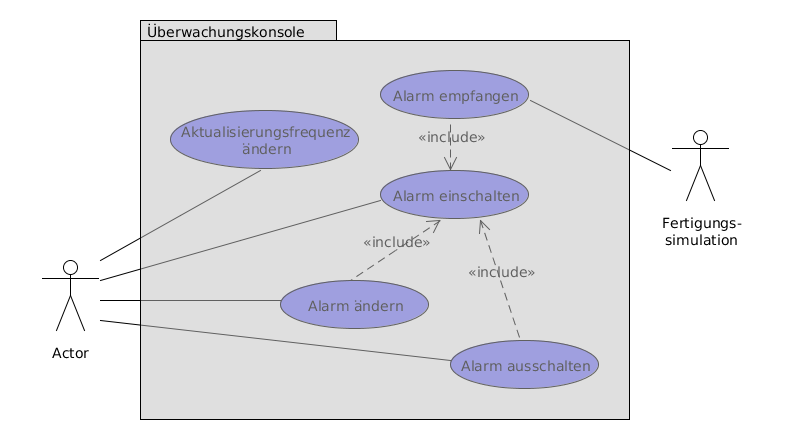
\includegraphics[scale=0.62]{media/UseCases/Ueberwachungskonsole.png}
  \caption{Anwendungsfalldiagramm für die Überwachungskonsole}
\end{figure}
\begin{figure}[H]
  \centering
  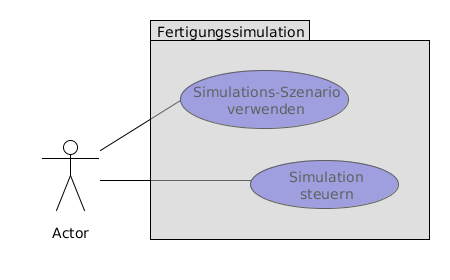
\includegraphics[scale=0.62]{media/UseCases/Fertigungssimulation.png}
  \caption{Anwendungsfalldiagramm für die Fertigungssimulation}
\end{figure}

\subsubsection{Änderung der Prozessvariablen}
\begin{description}
  \item[Name] Anpassen der Variablen wie Zu- oder Abflussgeschwindigkeit, Temperatur oder Motordrehzahl bei einem der
  Flüssigkeitstanks, sofern er die Anpassung dieser Werte erlaubt.
  \item[Akteure] Manuel (Bediener der Software)
  \item[Eingangsbedingung] Die \gls{Fertigungssimulation} und die \gls{Uberwachungskonsole} sind in Betrieb und miteinander verbunden.
  \item[Ereignisfluss]~\\
\begin{itemize}[noitemsep]
  \item Manuel öffnet das Steuerungsfenster.
  \item Manuel wählt den Reiter des Tanks, den er verändern will.
  \item Manuel stellt den gewünschten Wert ein.
  \item Manuel klickt den "`OK"' Knopf.
\end{itemize}
  \item[Ausgangssituation] Die \gls{Prozessvariable} ist geändert. Dies ist in der \gls{GUI} der \gls{Fertigungssimulation} sichtbar, etwa durch schnelleres Befüllen oder Leeren eines Tanks,
  durch ein schnelleres Drehen der Motorvisualisierung oder durch eine Statusanzeige.
    Außerdem zeigt die \gls{Uberwachungskonsole} die geänderte Variable an.
  \item [Nichtfunktionale Anforderungen] Die geänderte Variable wird mit der nächsten Aktualisierung auf der \gls{Uberwachungskonsole} angezeigt.
\end{description}

\subsubsection{Änderung der Verbindungseinstellungen}
\begin{description}
  \item[Name] Verändern der Verbindungseinstellungen.
  \item[Akteure] Manuel (Bediener der Software)
  \item[Eingangsbedingung] Die \gls{Fertigungssimulation} und die \gls{Uberwachungskonsole} sind in Betrieb und miteinander verbunden.
  \item[Ereignisfluss]~\\
  \begin{itemize}[noitemsep]
    \item Manuel öffnet in der \gls{Uberwachungskonsole} die allgemeinen Einstellungen.
    \item Manuel stellt die Aktualisierungsfrequenz, die \gls{IP-Adresse} oder einen Port der \gls{OPC UA Server} ein.
    \item Manuel klickt den "`Speichern"' Knopf und das Einstellungsfenster schließt sich.
    \item Der Verbindungsaufbau schlägt fehlt und das Einstellungsfenster öffnet sich wieder.
    \item Manuel trägt nun die richtigen Ports und \gls{IP-Adresse} ein und klickt erneut den "`Speichern"' Knopf.
  \end{itemize}
  \item[Ausgangssituation] Die \glspl{Sensordatum} in der \gls{Uberwachungskonsole} werden nun in Abständen der gewählten Aktualisierungsfrequenz aktualisiert.
  Wenn sich die \gls{IP-Adresse} oder Ports verändert haben, verbinden sich die betroffenen \glspl{OPC UA Client} neu mit dem Server.
  \item [Nichtfunktionale Anforderungen] Die Frequenz ändert sich spätestens mit der nächsten Aktualisierung.
\end{description}

\subsubsection{Erstes Starten der Simulation auf virtuellen Maschinen}
\begin{description}
  \item[Name] Einrichtung und Starten der Simulation auf virtuellen Maschinen.
  \item[Akteure] Manuel (Bediener der Software)
  \item[Eingangsbedingung] Ein Computer (oder virtuelle Maschine), auf der die .jar Datei der \gls{Uberwachungskonsole} gespeichert ist und ein Computer (oder virtuelle Maschine), auf der die .jar
    Datei der \gls{Fertigungssimulation} gespeichert ist, sind in Betrieb und haben feste \glspl{IP-Adresse} zugewiesen bekommen.
  \item[Ereignisfluss]~\\
  \begin{itemize}[noitemsep]
    \item Manuel startet die .jar der \gls{Fertigungssimulation}.
    \item Manuel startet die .jar der \gls{Uberwachungskonsole}.
    \item Manuel gibt die \gls{IP-Adresse} ein, unter der die \gls{Fertigungssimulation} zu finden ist.
  \end{itemize}
  \item[Ausgangssituation] Die \gls{Fertigungssimulation} und die \gls{Uberwachungskonsole} sind verbunden und laufen mit ihren Initialwerten.
\end{description}

\subsubsection{Alarm konfigurieren}
\begin{description}
  \item[Name] Einschalten, Ausschalten oder Konfigurieren des Schwellenwertes eines Alarms in der \gls{Uberwachungskonsole}.
  \item[Akteure] Manuel (Bediener der Software)
  \item[Eingangsbedingung] Die \gls{Fertigungssimulation} und die \gls{Uberwachungskonsole} sind in Betrieb und miteinander verbunden.
  \item[Ereignisfluss]~\\
  \begin{itemize}[noitemsep]
    \item Manuel \"offnet in der \gls{Uberwachungskonsole} die Alarmeinstellungen.
    \item Manuel schaltet einen Alarm ein oder aus, indem er die Checkbox anklickt, oder trägt einen Schwellwert ein.
    \item Manuel klickt den "`Speichern"' Knopf.
  \end{itemize}
  \item[Ausgangssituation] Wenn der Sensor die Alarmbedingung erf\"ullt und der Alarm aktiviert ist, wird an die \gls{Uberwachungskonsole} ein Alarm gesendet.
  Frühere Alarmschwellen lösen keine Alarme mehr aus.
\end{description}

\subsubsection{Alarm empfangen}
\begin{description}
  \item[Name] Empfangen eines (Überlauf-) Alarms in der \gls{Uberwachungskonsole}.
  \item[Akteure] Manuel (Bediener der Software)
  \item[Eingangsbedingung] Die \gls{Fertigungssimulation} und die \gls{Uberwachungskonsole} sind in Betrieb und miteinander verbunden.
    Es ist mindestens ein Überlauf-Alarm eingerichtet.
  \item[Ereignisfluss]~\\
  \begin{itemize}[noitemsep]
    \item In der \gls{Fertigungssimulation} kommt es zu einem Alarmzustand, weil ein Tank droht überzulaufen.
    \item Die \gls{Fertigungssimulation} sendet den entsprechenden Alarm an die registrierte \gls{Uberwachungskonsole}.
    \item Die \gls{Uberwachungskonsole} empf\"angt den Alarm.
    \item Die \gls{Uberwachungskonsole} zeigt in der \gls{GUI} den Alarm an, indem ein Dialog erscheint, die Ampel auf rot springt und der Kreis neben dem Wert ebenfalls rot wird.
    \item Da Manuel die Zuflussmengen der Tanks in der \gls{Fertigungssimulation} nicht reduziert, kommt es zu einem Überlauf.
    \item In der \gls{Fertigungssimulation} erscheint der Text "`Überlauf"' und Manuel klickt auf den "`Zurücksetzen"' Knopf.
    \item Die Fertigungssimulation wird in den Anfangszustand zurückgesetzt.
  \end{itemize}
  \item[Ausgangssituation] Die \gls{Uberwachungskonsole} läuft normal weiter und zeigt die zurückgesetzten Werte an. In der \gls{GUI} der
    \gls{Uberwachungskonsole} ist der Alarmeintrag zu sehen. Die \gls{Fertigungssimulation} ist auf den Anfangszustand zurück gesetzt.
\end{description}

\subsubsection{Ein Simulations-Szenario verwenden}
\begin{description}
  \item[Name] Starten eines \glslink{Simulations-Szenario}{Simulations-Szenarios}.
  \item[Akteure] Manuel (Bediener der Software)
  \item[Eingangsbedingung] Die \gls{Fertigungssimulation} und die \gls{Uberwachungskonsole} sind in Betrieb und miteinander verbunden.
  \item[Ereignisfluss]~\\
  \begin{itemize}[noitemsep]
    \item In der \gls{Fertigungssimulation} wird ein \gls{Simulations-Szenario} gestartet.
    \item Die \glspl{Prozessvariable} ändern sich deterministisch und ohne Zutun von Manuel. Diese Änderungen sind in der \gls{Uberwachungskonsole} sichtbar.
    \item Nachdem das \gls{Simulations-Szenario} fertig ist, wird die \gls{Fertigungssimulation} wieder auf den Anfangswert zurückgesetzt und das
    \gls{Simulations-Szenario} beginnt von vorne zu laufen.
    \item Manuel beendet das \gls{Simulations-Szenario} und die zuletzt vom \gls{Simulations-Szenario} eingestellten \glspl{Prozessvariable} können nun manuell von Manuel angepasst werden.
  \end{itemize}
  \item[Ausgangssituation] Das \gls{Simulations-Szenario} ist beendet. Es ändern sich keine \glspl{Prozessvariable} mehr automatisch.
\end{description}

\subsubsection{Verläufe konfigurieren}
\begin{description}
  \item[Name] Ein- oder Ausschalten eines Verlaufs.
  \item[Akteure] Manuel (Bediener der Software)
  \item[Eingangsbedingung] Die \gls{Fertigungssimulation} und die \gls{Uberwachungskonsole} sind in Betrieb und miteinander verbunden.
  \item[Ereignisfluss]~\\
  \begin{itemize}[noitemsep]
    \item Manuel öffnet die Verlaufseinstellungen in der \gls{Uberwachungskonsole}.
    \item Manuel klickt eine der Checkboxen.
    \item Manuel klickt den "`Speichern"' Knopf und das Einstellungsfenster schließt sich.
  \end{itemize}
  \item[Ausgangssituation] In der \gls{Uberwachungskonsole} wird der Verlauf des ausgewählten Wertes nun abhängig von der Checkbox angezeigt oder nicht angezeigt.
\end{description}


\subsection{Dynamische Modelle}
Für eine Erklärung der Elemente der folgenden Diagramme, siehe Abbildung \ref{explanation}
\begin{figure}[H]
  \centering
  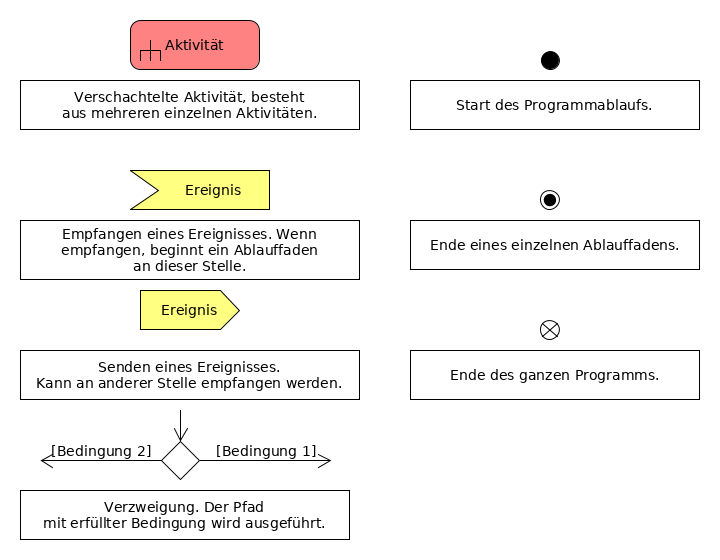
\includegraphics[scale=0.62]{media/Activities/explanation.png}
  \caption{Legende zu den Aktivitätsdiagrammen}
  \label{explanation}
\end{figure}

\subsubsection{Starten der Überwachungskonsole}
\label{console-launch}
\begin{figure}[H]
  \centering
  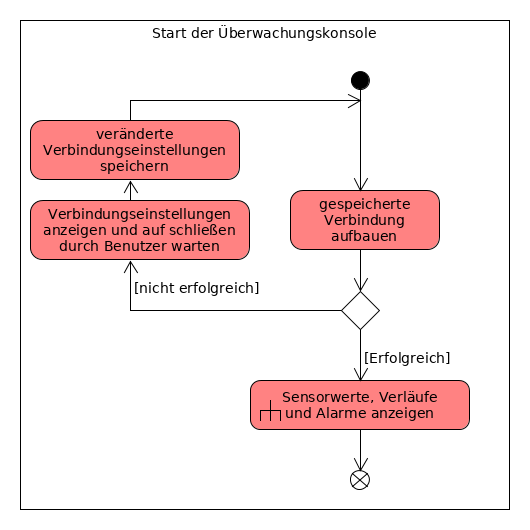
\includegraphics[scale=0.62]{media/Activities/launch-console.png}
  \caption{Aktivitätsdiagramm für den Start der Überwachungskonsole}
\end{figure}
\begin{enumerate}[noitemsep]
 \item Die \gls{Uberwachungskonsole} versucht, die Verbindung zu den \glslink{OPC UA Server}{OPC UA Servern} mit den zuletzt gespeicherten \glspl{Verbindungsinformation} aufzunehmen.
 \item Wenn der Verbindungsaufbau fehlschlägt, öffnet sich das Fenster mit den Verbindungseinstellungen. Wenn der Benutzer das Fenster wieder schließt,
 werden die veränderten \glspl{Verbindungsinformation} gespeichert und es wird erneut versucht, die Verbindung aufzubauen.
 \item Wenn der Verbindungsaufbau geklappt hat, zeigt die \gls{Uberwachungskonsole} die übertragenen Werte der \gls{Fertigungssimulation} sowie die
 Alarme und Verläufe an.
 \item Wenn der Benutzer die \gls{Uberwachungskonsole} schließt, ist das Programm beendet.
\end{enumerate}

\subsubsection{Hauptschleife und Alarme der Überwachungskonsole}
\begin{figure}[H]
  \centering
  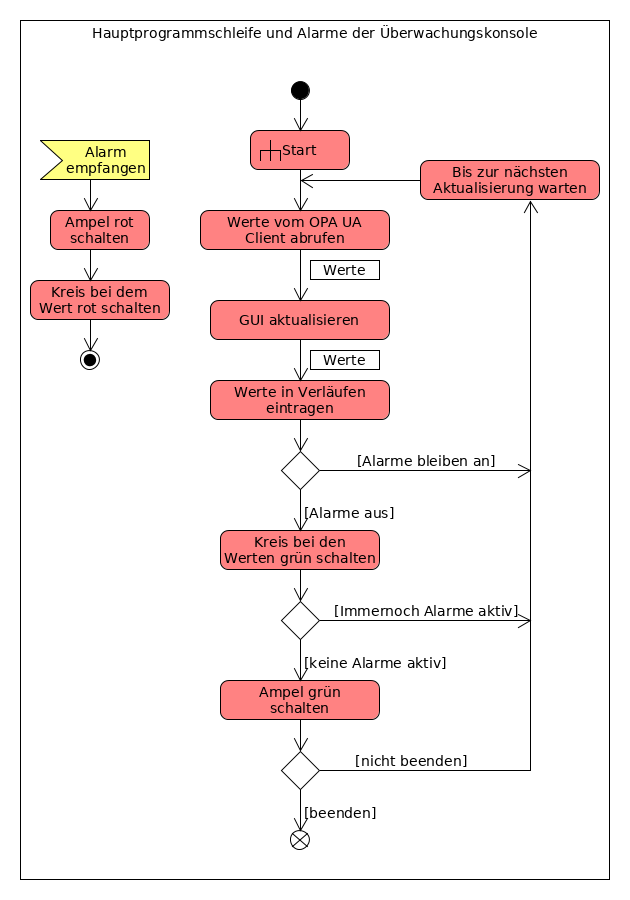
\includegraphics[scale=0.62]{media/Activities/main-console.png}
  \caption{Aktivitätsdiagramm für die Hauptschleife und Alarme der Überwachungskonsole}
\end{figure}

\emph{Hauptschleife}
\begin{enumerate}[noitemsep]
 \item Die \gls{Uberwachungskonsole} startet, wie in \ref{console-launch} beschrieben.
 \item Die \gls{Uberwachungskonsole} ruft die aktuellen Sensorwerte vom \gls{OPC UA Server} ab.
 \item Diese Werte werden auf den Anzeigen der \gls{Uberwachungskonsole} angezeigt.
 \item Dann werden diese Werte in den Verlauf (sofern aktiviert) eingefügt.
 \item Wenn bei einem aktivem Alarm die Alarmbedingung nicht mehr erfüllt ist, wird er ausgeschaltet.
 \item Wenn keine Alarme mehr aktiv sind, wird die Ampel auf grün geschaltet.
 \item Wenn der Benutzer das Fenster geschlossen hat, wird die \gls{Uberwachungskonsole} beendet.
 \item Vor der nächsten Aktualisierung wird gewartet, damit erst nach der Aktualisierungsfrequenz erneut Sensorwerte abgerufen werden.
\end{enumerate}
\emph{Alarme empfangen}
\begin{enumerate}[noitemsep]
 \item Wenn ein Alarm empfangen wird, wird die Ampel auf rot geschaltet.
 \item Dann wird der Kreis bei den Anzeigen auf rot geschaltet.
\end{enumerate}

\subsubsection{Hauptschleife der Fertigungssimulation}
\begin{figure}[H]
  \centering
  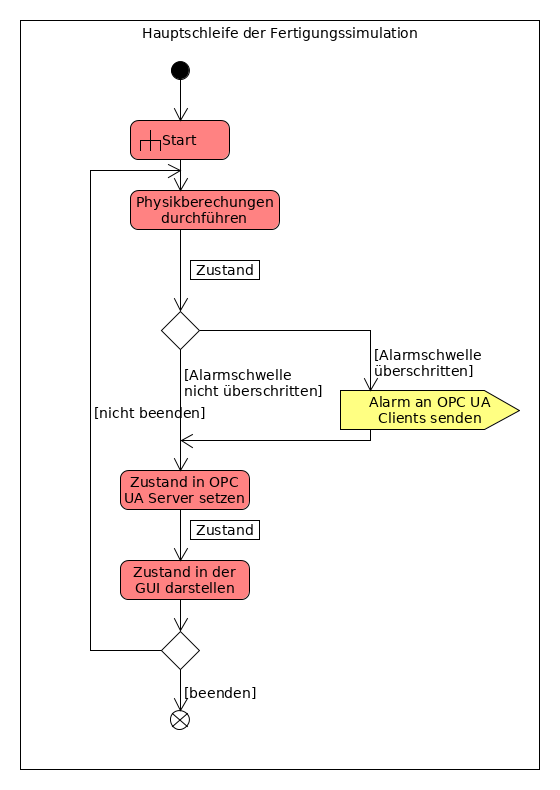
\includegraphics[scale=0.62]{media/Activities/main-simulation.png}
  \caption{Aktivitätsdiagramm für die Hauptschleife der Fertigungssimulation}
\end{figure}

\begin{enumerate}[noitemsep]
 \item Die \gls{Fertigungssimulation} startet.
 \item Der Zustand der \gls{Fertigungssimulation} wird berechnet.
 \item Wenn durch eine Zustandsänderung eine Alarmschwelle überschritten wurde, wird der Alarm an alle \glspl{OPC UA Client} gesendet,
 die sich für den Alarm registriert haben.
 \item Danach wird der geänderte Zustand im \gls{OPC UA Server} gesetzt.
 \item Dann wird der aktualisierte Zustand in der \gls{GUI} angezeigt.
 \item Wenn der Benutzer das Fenster geschlossen hat, wird die \gls{Fertigungssimulation} beendet.
\end{enumerate}

\subsection{Statische Modelle}
\subsubsection{Komponentendiagramm}
\begin{figure}[H]
  \centering
  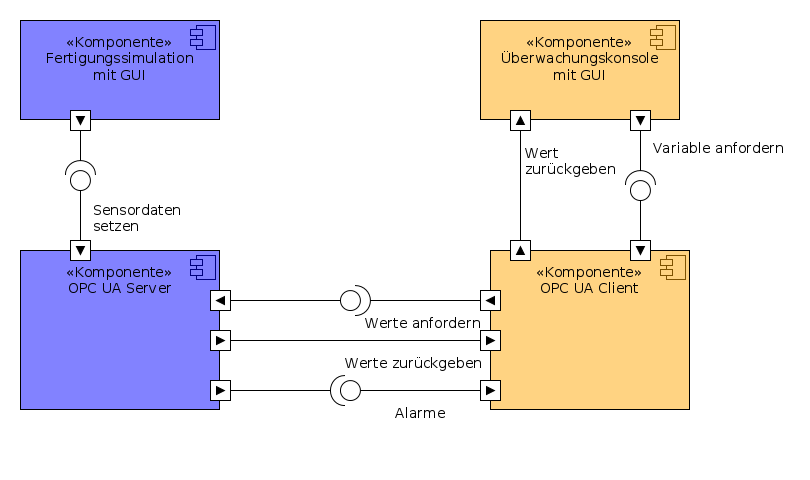
\includegraphics[scale=0.5]{media/ComponentDiagram/componentDiagram.png}
  \caption{Komponentendiagramm}
\end{figure}

Die \gls{Fertigungssimulation} simuliert die Werte f\"ur die Tanks. Sie zeigt in ihrer \gls{GUI} eine schematische Darstellung der
\gls{Produktionsanlage}. Die \gls{Produktionsanlage} l\"asst sich \"uber die \gls{Fertigungssimulation} steuern. Die \gls{Fertigungssimulation} setzt
in den \glslink{OPC UA Server}{OPC UA Servern} die "`gemessenen"' Sensorwerte.

Die \glspl{OPC UA Server} aggregieren mehrere \glspl{Sensordatum}, die durch die \gls{Fertigungssimulation} gesetzt werden. An jedem \gls{OPC UA Server} k\"onnen
sich beliebig viele \glspl{OPC UA Client} registrieren. Auf Anfrage erhalten die \glspl{OPC UA Client} \glspl{Sensordatum}. Bei einem \gls{OPC UA Server} registrierte
Alarme werden an die \glspl{OPC UA Client} geschickt, wenn ausgelöst.

Die \glspl{OPC UA Client} sind bei je genau einem \gls{OPC UA Server} registriert. Sie fragen, wenn sie von der \gls{Uberwachungskonsole} dazu
aufgefordert werden, die Daten von ihrem jeweiligen \gls{OPC UA Server} ab. Sie k\"onnen bei ihrem \gls{OPC UA Server} Alarme registrieren und diese
dann empfangen. Die \glspl{OPC UA Client} stellen der \gls{Uberwachungskonsole} Daten bereit.

Die \gls{Uberwachungskonsole} verwendet vier \glspl{OPC UA Client}, um \"uber diese und die \glspl{OPC UA Server} Daten von der
\gls{Fertigungssimulation} zu erhalten. \"Uber die \gls{Uberwachungskonsole} werden die \glspl{OPC UA Client} indirekt gesteuert.
Es werden intern vier \glspl{OPC UA Client} benutzt, da jeder der Clients nur mit einem einzelnen Endpunkt kommunizieren kann.
In der \gls{Uberwachungskonsole} kann der Benutzer Alarme
f\"ur die \glspl{OPC UA Client} registrieren und angeben, welche Daten von den \glslink{OPC UA Server}{OPC UA Servern} abgefragt werden sollen. Die Daten und Alarme, die
die \gls{Uberwachungskonsole} von den \glspl{OPC UA Client} erh\"alt, stellt sie graphisch dar.

Die einzige Verbindung von \gls{Uberwachungskonsole} und \gls{Fertigungssimulation} ist \"uber die \glspl{OPC UA Server} und \glspl{OPC UA Client} realisiert.

\section{Nutzerinterface-Skizzen}
\subsection{Fertigungssimulation}
\begin{figure}[H]
  \centering
  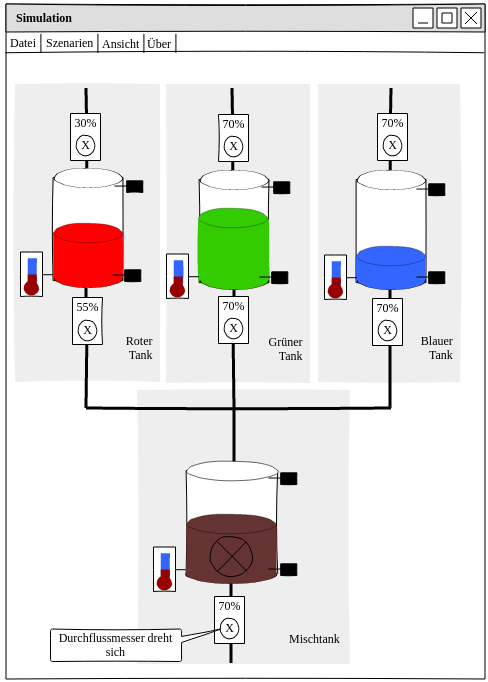
\includegraphics[scale=0.5]{media/ui-server/ui-server-main.png}
  \caption{Nutzerinterface-Skizze des Hauptfensers der Fertigungssimulation}
\end{figure}
Im Hauptfenster der \gls{Fertigungssimulation} wird die simulierte \gls{Produktionsanlage} angezeigt. Dabei wird jeder der Tanks
mit einem blassgrauen Kasten hinterlegt, um den Zuständigkeitsbereich der einzelnen \gls{OPC UA Server} abzugrenzen. Die Anzeige wird
in Echtzeit von der Simulation aktualisiert. Die Anzeigen der Durchflussmesser sowie der Motor im unteren Tank drehen sich.
Die Tanks werden als Zylinder dargestellt, die in der entsprechenden Farbe gefüllt sind.

\begin{figure}[H]
  \centering
  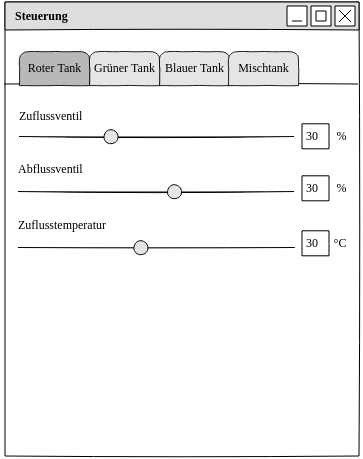
\includegraphics[scale=0.5]{media/ui-server/ui-server-control.png}
  \caption{Nutzerinterface-Skizze des Steuerungsfensters der Fertigungssimulation}
\end{figure}
Über das Menü kann ein Fenster angezeigt werden, das die Konfiguration der einzelnen \glspl{Prozessvariable} erlaubt. Hierbei
wird für den Zuständigkeitsbereich jedes \glslink{OPC UA Server}{OPC UA Servers} ein Reiter angezeigt. Die Reiter beziehen sich also
direkt auf die dargestellten blassgrauen Kästen. Die Einstellungen der jeweiligen \glspl{Prozessvariable} erfolgt über Schieberegler.

\begin{figure}[H]
  \centering
  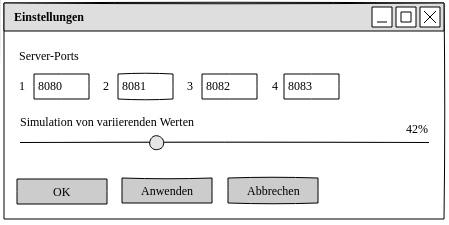
\includegraphics[scale=0.5]{media/ui-server/ui-server-settings.png}
  \caption{Nutzerinterface-Skizze des Einstellungsfensters der Fertigungssimulation}
\end{figure}
Im Einstellungsdialog können die Ports der jeweiligen Server über Textfelder eingestellt werden. Der \gls{Jitter} kann über einen Schieberegler
eingestellt werden. Es existieren die Buttons "`Abbrechen"' und "`OK"'.

\pagebreak

\subsection{Überwachungskonsole}
\begin{figure}[H]
  \centering
  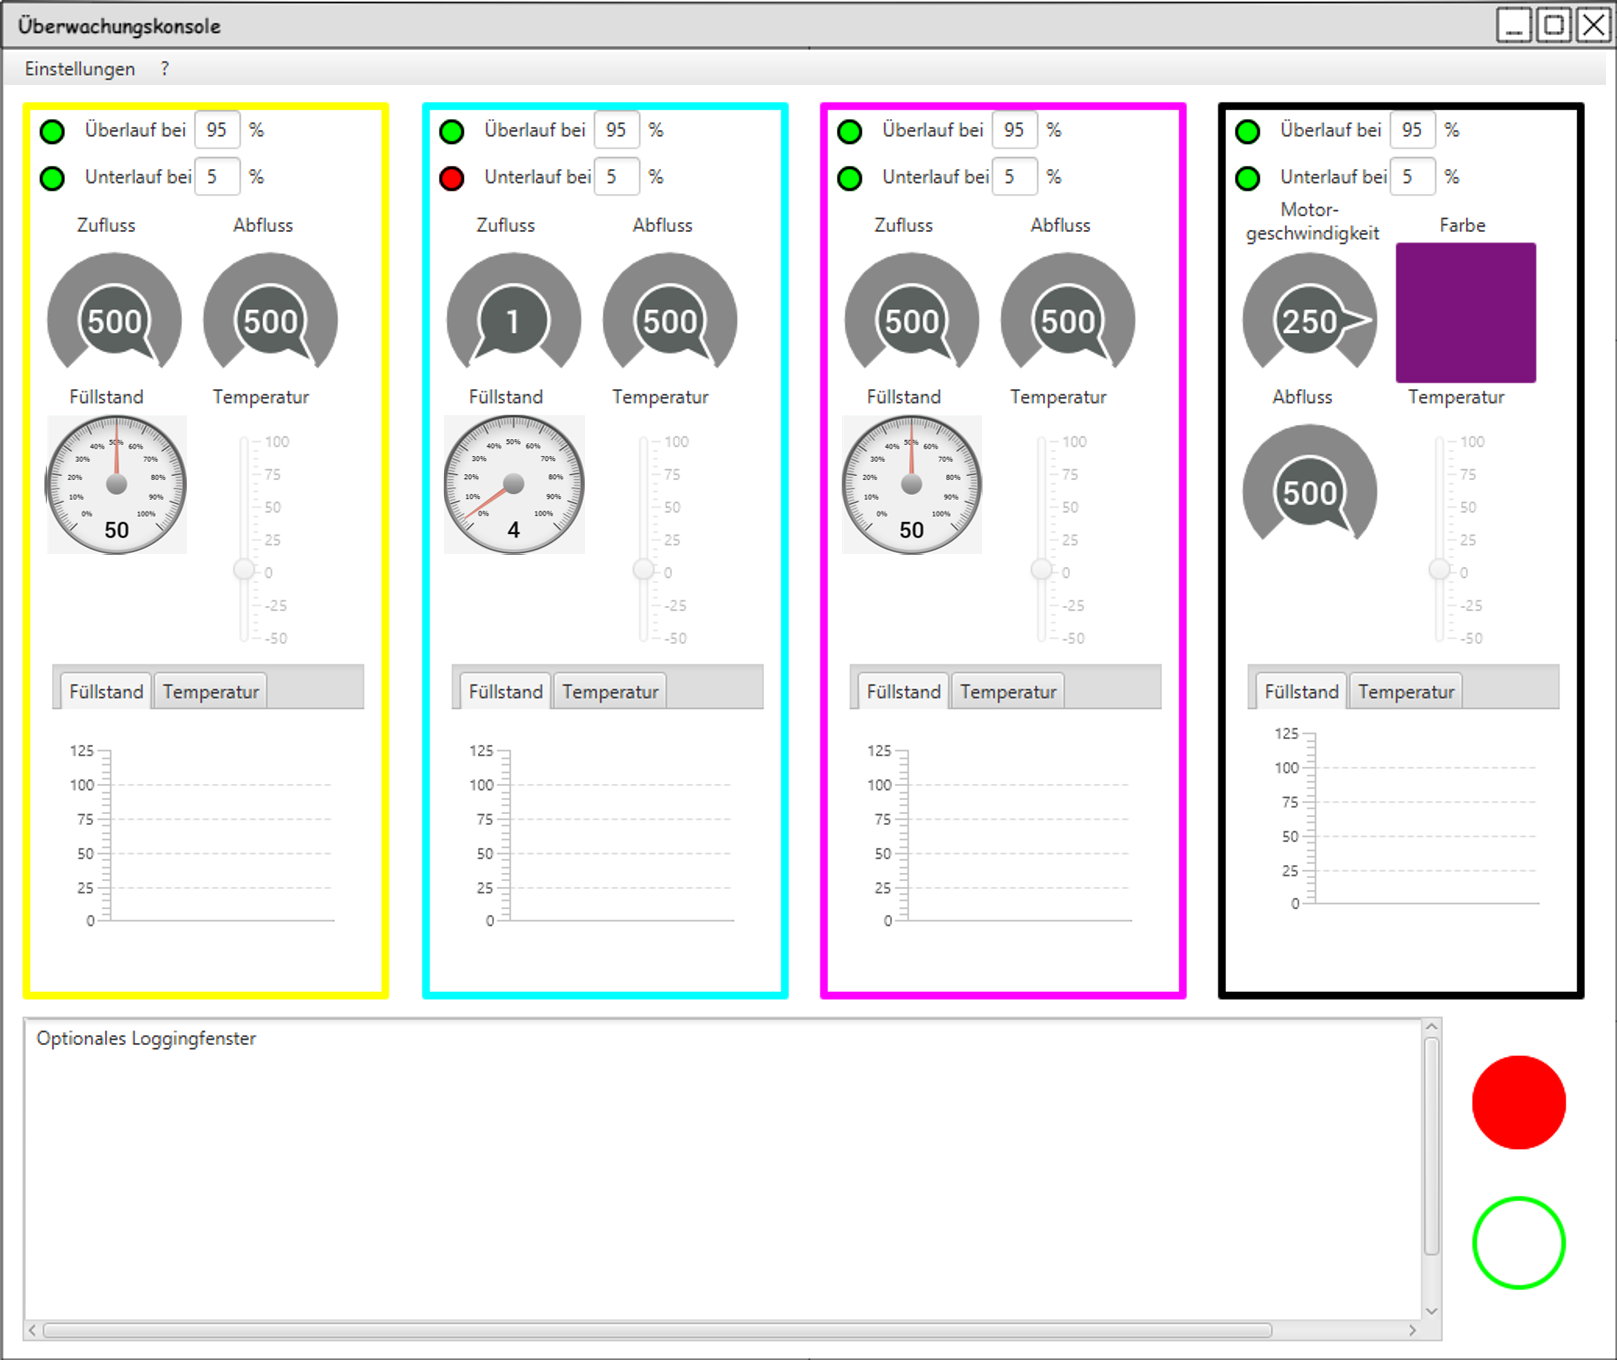
\includegraphics[scale=0.35]{media/ui-client/ui-uw.png}
  \caption{Nutzerinterface-Skizze des Hauptfensters der Überwachungskonsole}
\end{figure}
Im Hauptfenster der \gls{Uberwachungskonsole} werden die Anzeigen für die \glspl{Sensordatum} für jeden Tank in einem einzelnen Rahmen gesammelt. Dabei repräsentieren die Anzeigen im gelben, cyanfarbenen bzw.
magentafarbenen Rahmen den gelben, cyanfarbenen bzw. magentafarbenen Tank. Die Anzeigen im schwarzen Rahmen repräsentieren den Mischtank, dessen Farbe explizit angezeigt wird.
Neben den Anzeigen der \glspl{Sensordatum} sind auch die Füllstands- und Temperaturverläufe in Form von Diagrammen und die Alarme enthalten. Im cyanfarbenen Tank ist beispielhaft der Alarm für einen Unterlauf ausgelöst.
Darüber hinaus enthält das Hauptfenster das Loggingfenster und die Ampel für den allgemeinen Zustand der \gls{Uberwachungskonsole}.

\begin{figure}[H]
	\centering
	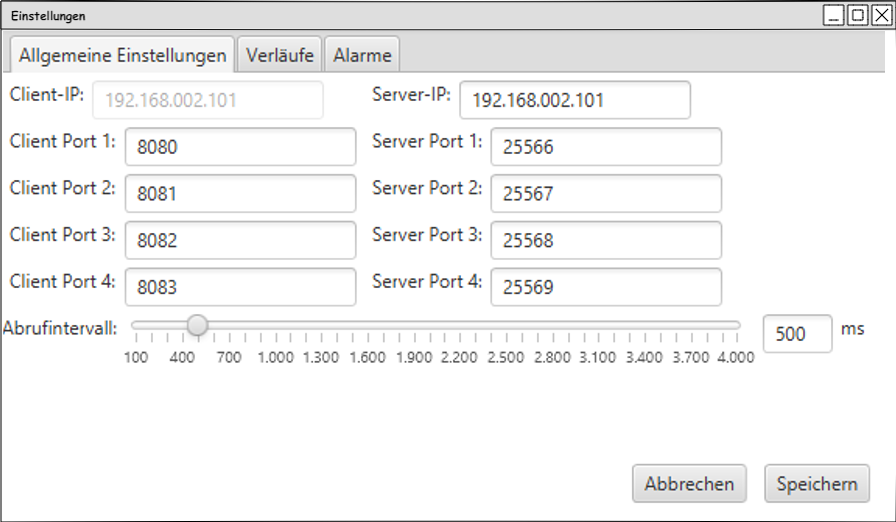
\includegraphics[scale=0.3]{media/ui-client/ui-uw-settings1.png}
	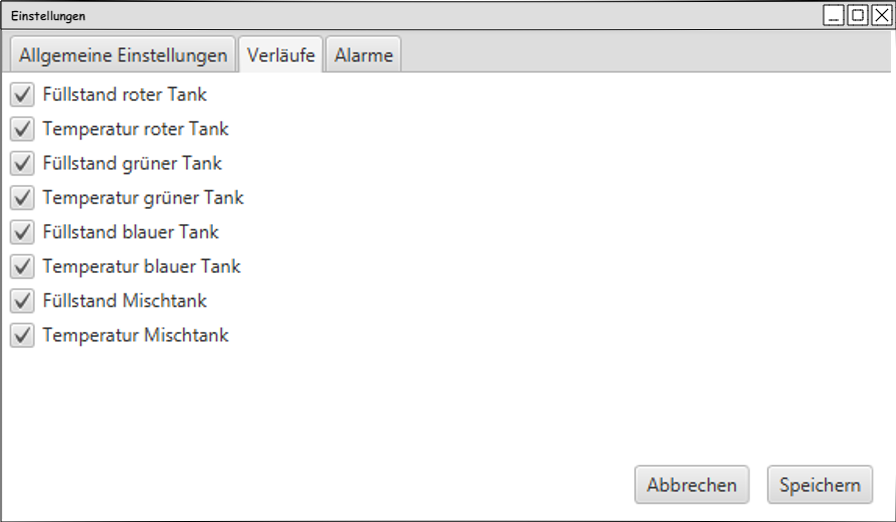
\includegraphics[scale=0.3]{media/ui-client/ui-uw-settings2.png}
	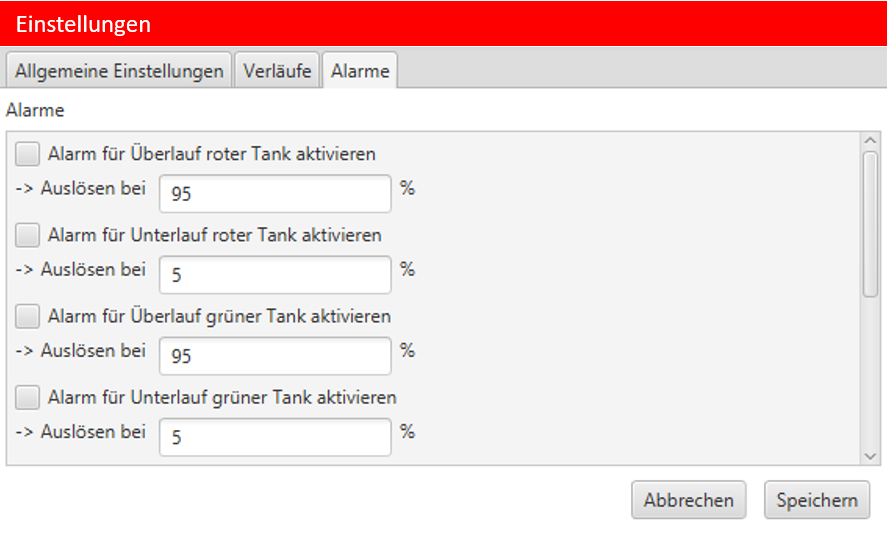
\includegraphics[scale=0.3]{media/ui-client/ui-uw-settings3.png}
	\caption{Nutzerinterface-Skizze des Einstellungsdialogs der Überwachungskonsole}
\end{figure}
Im Einstellungsdialog sind bereits alle möglichen Einstellungen skizziert. Dem entsprechend beinhalten die "`Allgemeinen Einstellungen"' die \glspl{Verbindungsinformation}, die Sprache und die Aktualisierungsfrequenz, die "`Verläufe"' das Ein- und Ausschalten der einzelnen Füllstands- und Temperaturverläufe und die "`Alarme"' das Einstellen dieser.

\begin{figure}[H]
	\centering
	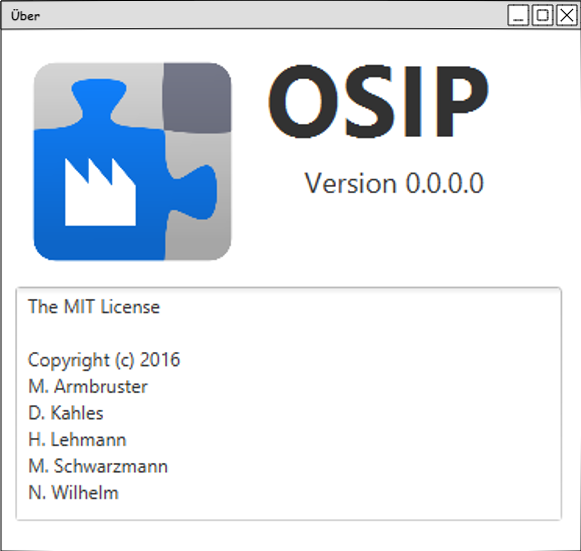
\includegraphics[scale=0.4]{media/ui-client/ui-uw-uber.png}
	\caption{Nutzerinterface-Skizze des "`Über"'-Fensters der Überwachungskonsole}
\end{figure}
Das "`Über"'-Fenster der \gls{Uberwachungskonsole} enthält die Programm- und Lizenzinformationen zum Projekt. Daneben bietet es im Lizenztextfeld Platz für die Lizenzen verwendeter Bibliotheken; es kann aber auch um ein separates Feld für diese Lizenzen erweitert werden.

\pagebreak
\printglossaries

\pagebreak
\phantomsection
\addcontentsline{toc}{section}{\listfigurename}
\listoffigures

\end{document}
